\documentclass[UTF8]{EPURapport}
%\usepackage{listings}

%\renewcommand{\lstlistlistingname}{Liste des codes}
%\renewcommand{\lstlistingname}{Code}

%\addextratables{%
%	\lstlistoflistings
%}

%\swapAuthorsAndSupervisors

\thedocument{Manuel administrateur}{Canne connectée pour aveugles}{}
\grade{Département Informatique\\ 5\ieme{} année\\ 2020-2021}
\authors{%
	\category{Auteurs}{%
		\name{Djawad M'DALLAH MARI} \mail{djawad.mdallah-mari@etu.univ-tours.fr}
	}
	\details{DII5 2020-2021}
}
\supervisors{%
	\category{Encadrants}{%
		\name{Gilles VENTURINI} \mail{gilles.venturini@etu.univ-tours.fr}
	}
	\details{Université François-Rabelais, Tours}
}
\abstracts{Manuel administrateur canne connecée pour aveugles}
{}
{}
{}

\begin{document}

\chapter{Introduction}

Ce document fait partie d'un ensemble de livrables qui accompagne le projet de fin d'études "Canne connectée pour aveugles" réalisé en 2020-2021 à Polytech Tours par Djawad M'DALLAH-MARI.\\

C'est un manuel administrateur qui vise toute personne souhaitant obtenir plus d'information sur la configuration du système, son installation, son déploiement et toutes autres tâches qui incombe à l'administration du système.

\chapter{Déploiement}
Dans ce chapitre nous verrons comment obtenir l'application et comment le déployer afin qu'il soit accessible aux utilisateurs finaux.

\section{Génération de l'APK}

Il faut tout d'abord récupérer le code source du projet disponible sur le github \footnote{\url{https://github.com/Djawad-mdallahmari/PFE-ObjectDetection}}. Une fois le code cloner, il faut l'ouvrir avec Android Studio (voir installation Android Studio \footnote{\url{https://developer.android.com/studio/install}}). Après avoir vérifié que le code compile bien (se référrer au manuel mainteneur), il faut générer le .apk (Android Package). C'est le format de fichier de package utilisé par Android. C'est ce qui va permettre d'archiver le programme avec tous ces ressources dans un seul fichier qui pourra être déployer facilement par la suite.\\
Pour générer un APK de manière rapide (pour des tests par exemple) il suffit de cliquer sur \verb|Build >  Build Bundle(s) / APK(s) > Build APK(s)|. Un fichier avec l'extension .apk sera générer dans le dossier \verb|PFE-ObjectDetection\app\build\outputs\apk\interpreter\debug| et pourra donc être utiliser directement. Cependant, pour déployer l'application sur le Play Store par exemple il est préférable de générer l'APK autrement car l'application sera plus adapté et aura une taille moins importante. Pour cela, il faut cliquer sur \verb|Build > Generate Signed Bundle or APK| et suivre les instructions jusqu'à la génération de l'APK.

\begin{figure}[h!]
\centering
  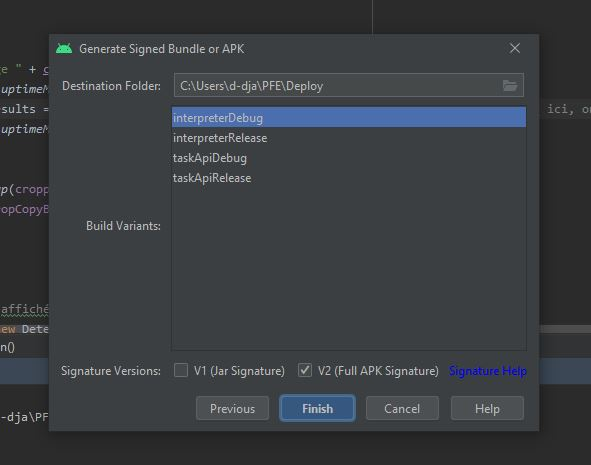
\includegraphics[width=0.3\textwidth]{images/generateAPK.jpg}
  \caption{Génération de l'APK}
  \label{fig:genapk}
\end{figure}

\section{Google Play Console}

Après avoir généré l'APK, nous pouvons désormais le déployer sur le Google Play. Pour cela, il faut disposer d'un compte Google Play Console \footnote{\url{https://play.google.com/console/about/}}. Une fois connectée sur la plateforme, il faut aller sur créer une application et suivre les instructions.

\begin{figure}[h!]
\centering
  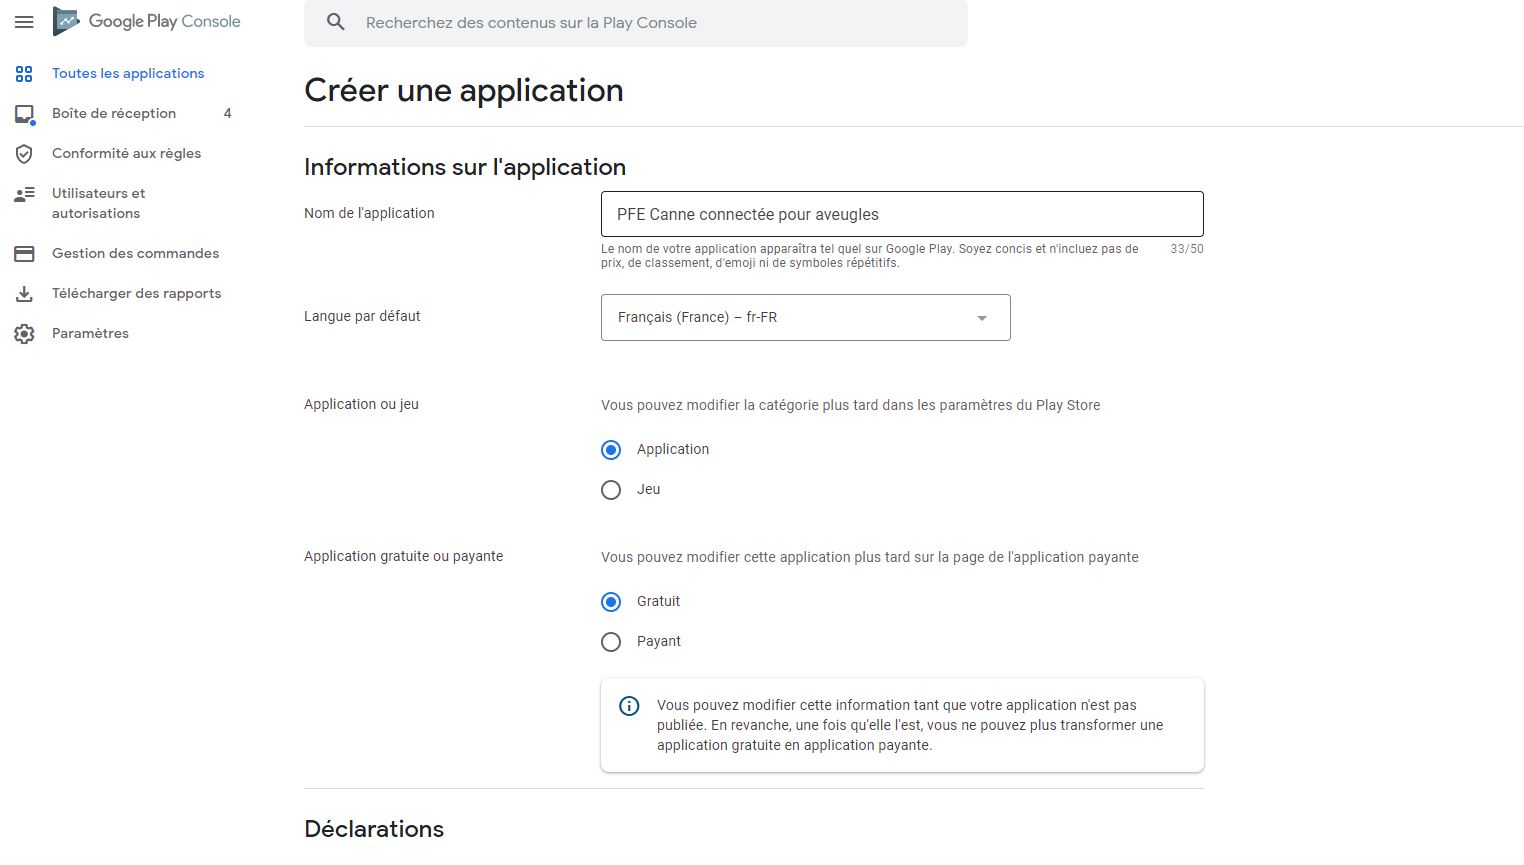
\includegraphics[width=0.3\textwidth]{images/CreateAppConsole.JPG}
  \caption{Creation de l'application sur Google Play Console}
  \label{fig:createappconsole}
\end{figure}

On attérit sur une section avec des menus spécifique à l'application qu'on souhaite déployer. Il faut ensuite aller sur le menu Production puis déposer le fichier .apk généré précedemment.

\begin{figure}[h!]
\centering
  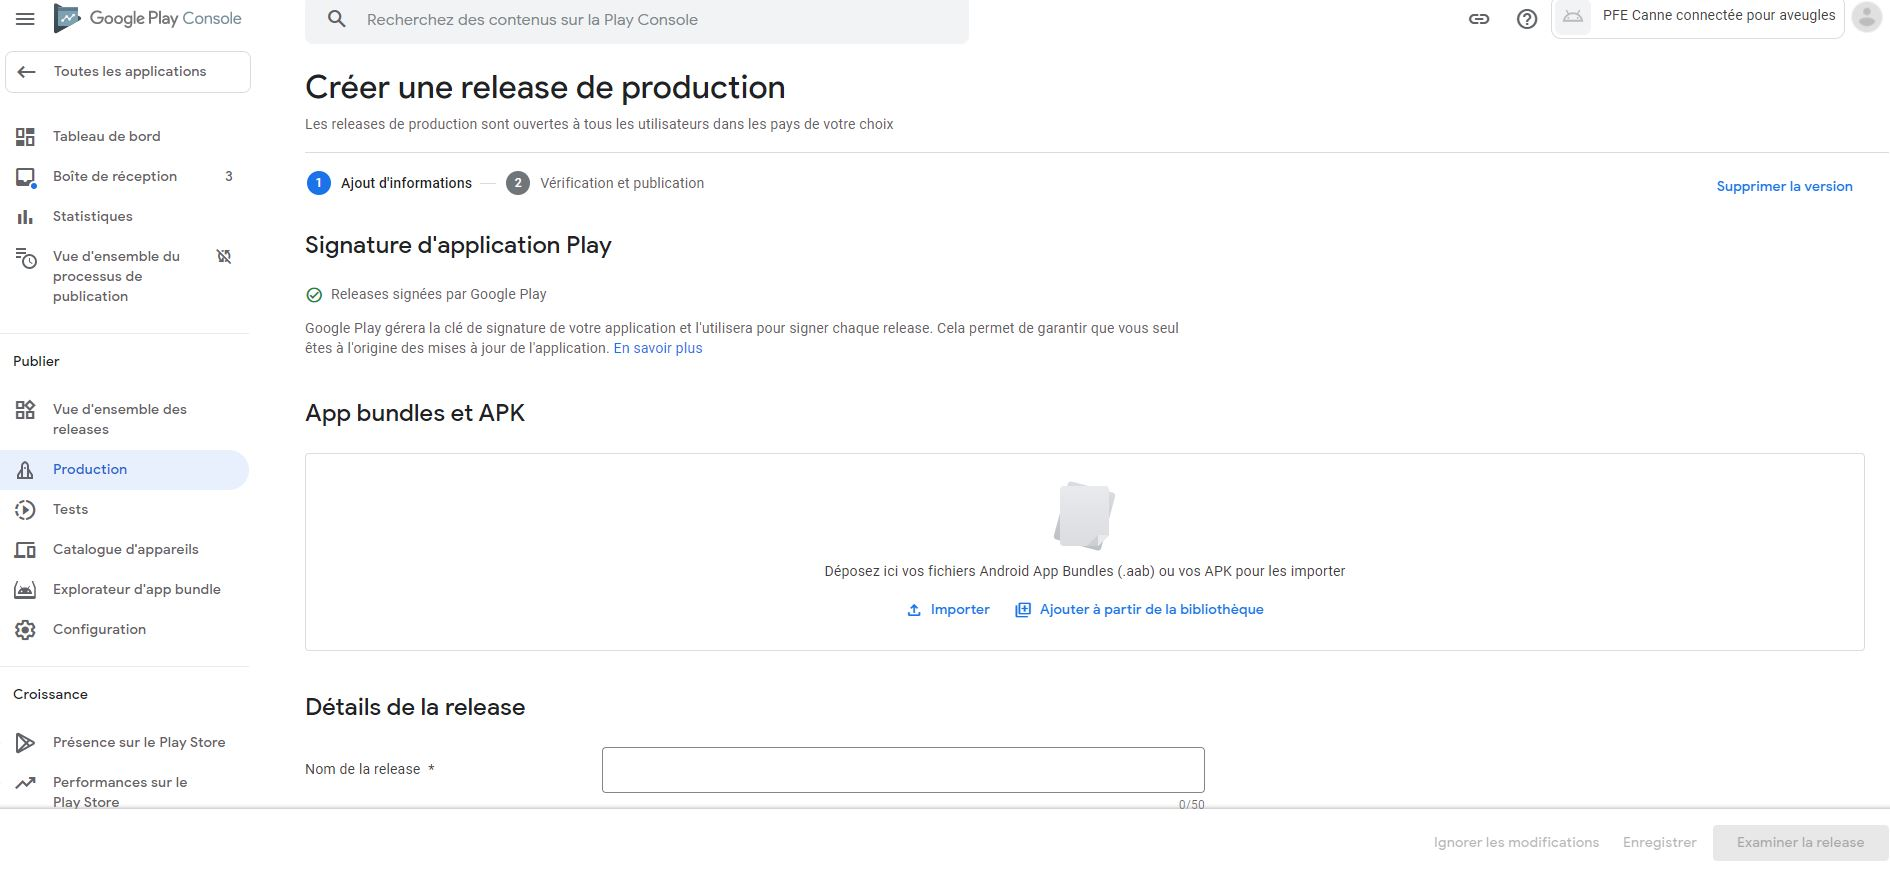
\includegraphics[width=0.3\textwidth]{images/release.JPG}
  \caption{Dépôt de l'APK sur Google Play Console}
  \label{fig:depotapk}
\end{figure}

Une fois effectué l'application ne sera pas encore disponible sur le Google Play, il faudra attendre que les vérifications soient terminées. Si l'application est conforme aux politiques de Google, il sera publier par la suite sur le Google Play.

\section{Vérification du déploiement}
La dernière étape du déploiement est la vérification de la disponibilité de l'application sur le Google Play. Pour cela il suffit de se rendre sur le Google Play et rechercher le nom de l'application. L'application devrait apparaître parmis la liste des résultats de recherche.

\chapter{Installation}
\section{Installation depuis Google Play}
télécharger
\section{Installation depuis l'APK}
.apk, source inconnu
\section{Installation depuis Android Studio}
fleche verte
\chapter{Configuration}
\section{vérification des configurations}
par défaut pas mute, seuil de détection, 

\annexes

\end{document}